\section{Introduction} 
\subsection{Problem Statement}

In this project we are trying to classify 3D point cloud. The data set is sets of \emph{point clouds}. Each point cloud is comprised of a set of $n$ data points. A data point is a tuple of 3D coordinates ($x,y,z$) of the point in the space. Figure ~\ref{fig:ex} shows few examples of the data set we have. Each point cloud is associated with a label shown under the model. 


The data set (ModelNet40 \citep{wu20153d}) consists of 9840 point clouds for training and 2468 point clouds for testing. Our task is to create a CNN model that can train such data set and achieve good accuracy within the test point cloud. 

\begin{figure}[hbt]
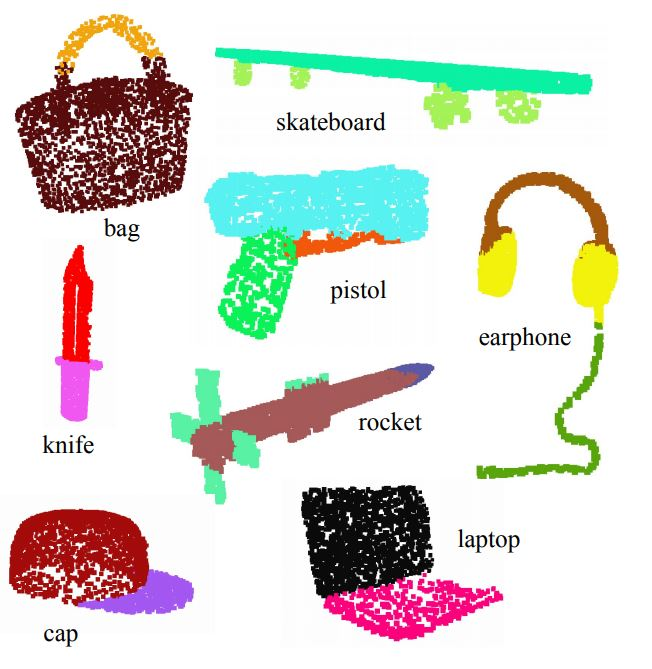
\includegraphics[height=2.5in, width=2.5in]{fig/ex.JPG}
\caption{Example point clouds (color here are added for visualization only).}
\label{fig:ex}
\end{figure}


\subsection{Challenges}
At first glance the classification looks similar to classifying images which has been investigated thoroughly in the past couple of years. However, with a careful look at the problem and the type of input we have, we can realize the following challenges that will influence our model
\paragraph{Irregularity:}
While standard deep neural network models take as input data with regular structure (images of a fixed sizes), point clouds are irregular. This means we have no expectation on the input size (the number of points per point cloud). The reason behind this is that these point clouds either come from scan operations or hand-crafted which can not be constrained to give point cloud of fixed size.

\paragraph{Unordered:} Point positions are continuously distributed in the space and any permutation to their ordering does not change the spatial distribution. The point cloud is read from a file which could store the point in a certain order that is different than other point cloud models. Thus, associating the feature with the point order could be misleading.
\paragraph{Invariance:} The learned features should be invariant to translation and rotation. Our model should be able to accurately classify similar point cloud even if they are rotated or shifted. Similar case exists in images where a certain feature could be located anywhere in the image. However, with point cloud in 3D space the problem is augmented as there is a third degree of freedom for translation and rotation. 

\begin{figure*}[!tbh]
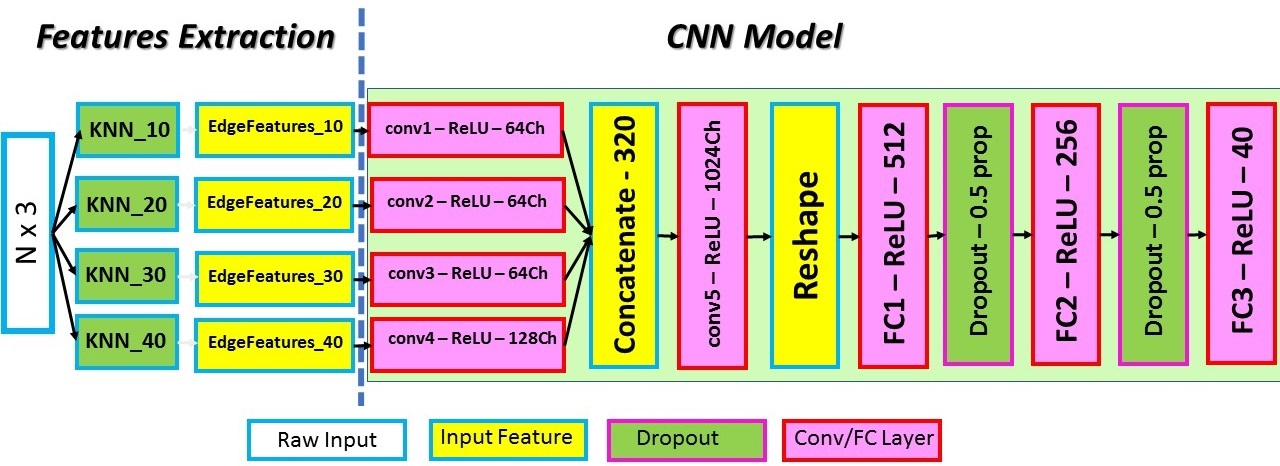
\includegraphics[width=1.0\textwidth]{fig/model1.JPG}
\caption{The main components of our model. Feature extraction is responsible of extracting global and local feature from the point cloud where the CNN model is the training model.}
\label{fig:model1}
\end{figure*}


\subsection{Previous Work}
Previous work on point cloud classification using CNN has three main directions:
\paragraph{View-based Methods:}
These methods represent a single model as a collection of 2D views to which standard CNNs used in image classification can be employed directly. View-based appraoches are good match for applications where the input comes from 3D sensor and represented as a range image in which case a single view can be used~\citep{wei2016dense}. 

\paragraph{Volumetric Methods:}
Voxelization is another straightforward way to convert irregular data set to a regular 3D grid over which standard CNN can be applied~\citep{maturana2015voxnet}. However, voxelization produces a sparsely-occupied grids and induce quantization artifacts. Cleverer space partition like $k$-d tree can be used to mitigate these problems~\citep{klokov2017escape}.
\paragraph{Direct Methods:}
These methods try to learn from the raw data points without voxelization or alternating the views. It should be expected that these methods to have greater accuracy since we do not manipulate the feature being learned. However, proper model design is challenging due to the challenges been mention earlier. The pioneer work on tackling point cloud learning from the raw data set is PointNet~\citep{pointnet}. PointNet applies a symmetric function to the 3D coordinates in a manner invariant to permutation where every point is treated individually. However, PointNet employs a complex and computationally expensive spatial transformer network to learn the 3D alignment of the points. This is due to the fact that the feature being learned are global features and no local features are utilized.  